\subsection{Wąskie gardło}
Następny szukamy przekroju o jak najmniejszej przepustowości \\
W tym celu usunęliśmy parametry dotyczące średniego zużycia dobowego oraz kosztów transportu i zostawiliśmy wyłącznie przepustowość
\begin{lstlisting}[caption= plik dat]
data; 
 
set BudynkiNaStart := s, A, B, C, D, E, F, G, H; 
set Budynki := A, B, C, D, E, F, G, H; 
set Elektrownie := F, G, H; 
 
param p := 
s A 10 s B 13 s C 17 s D 0  s E 0  s F 0  s G 0  s H 0
A A 0  A B 0  A C 0 A D 15  A E 10 A F 0  A G 0  A H 0
B A 0  B B 0  B C 0 B D 4 B E 9  B F 0  B G 9  B H 0
C A 0  C B 0 C C 0 C D 20 C E 10 C F 0  C G 0  C H 0   
D A 0  D B 0  D C 0  D D 0 D E 0 D F 10 D G 3   D H 2 
E A 0  E B 0  E C 0 E D 20 E E 0 E F 5 E G 5  E H 5  
F A 0  F B 0  F C 0  F D 0  F E 0  F F 0  F G 0  F H 0
G A 0  G B 0  G C 0 G D 0  G E 0  G F 0  G G 0  G H 0
H A 0  H B 0  H C 0  H D 0  H E 0  H F 0  H G 0 H H 0; 
 
end; 
\end{lstlisting}
\begin{lstlisting}[caption= plik mod]
set BudynkiNaStart; 
set Budynki; 
set Elektrownie; 
 
param p{i in BudynkiNaStart, j in Budynki}; 
 
var f{i in BudynkiNaStart, j in Budynki}, >= 0; 
 
maximize Q: sum {i in Budynki, e in Elektrownie} f[i,e]; 
 
subject to 
  Ograniczenie_jeden{i in BudynkiNaStart, j in Budynki}: 
    f[i,j] >= 0; 
  Ograniczenie_dwa{i in BudynkiNaStart, j in Budynki}: 
    f[i,j] <= p[i,j]; 
  Ograniczenie_trzy{n in Budynki}: 
    sum {i in Budynki} f[n,i] <= sum {j in BudynkiNaStart} f[j,n]; 
 
solve; 
display {i in Budynki, j in Budynki: f[i,j] > 0}: f[i,j]; 
display: Q;
\end{lstlisting}

\paragraph{Wyniki}
\begin{lstlisting}[caption=Wynik z glpk]
f[A,D].val = 9
f[A,E].val = 1
f[B,E].val = 4
f[B,G].val = 9
f[C,D].val = 6
f[C,E].val = 10
f[D,F].val = 10
f[D,G].val = 3
f[D,H].val = 2
f[E,F].val = 5
f[E,G].val = 5
f[E,H].val = 5
Q.val = 39
\end{lstlisting}

\begin{figure}[htb]
\caption{Wyniki poszukiwań wąskiego gardła}
\begin{center}
\begin{tabular}{ | c | c | c | c | c | c | }
\hline
  & D & E & F & G & H \\ 
 \hline
 A & 9 & 1 & - & - & -\\  
 \hline
 B & - & 4 & - & 9 & - \\
 \hline  
 C & 6 & 10 & - & - & - \\
 \hline  
 D & - & - & 10 & 3 & 2 \\
 \hline  
 E & - & - & 5 & 5 & 5 \\
 \hline  
\end{tabular}
\end{center}
\end{figure}

\[ Q = 39 \]

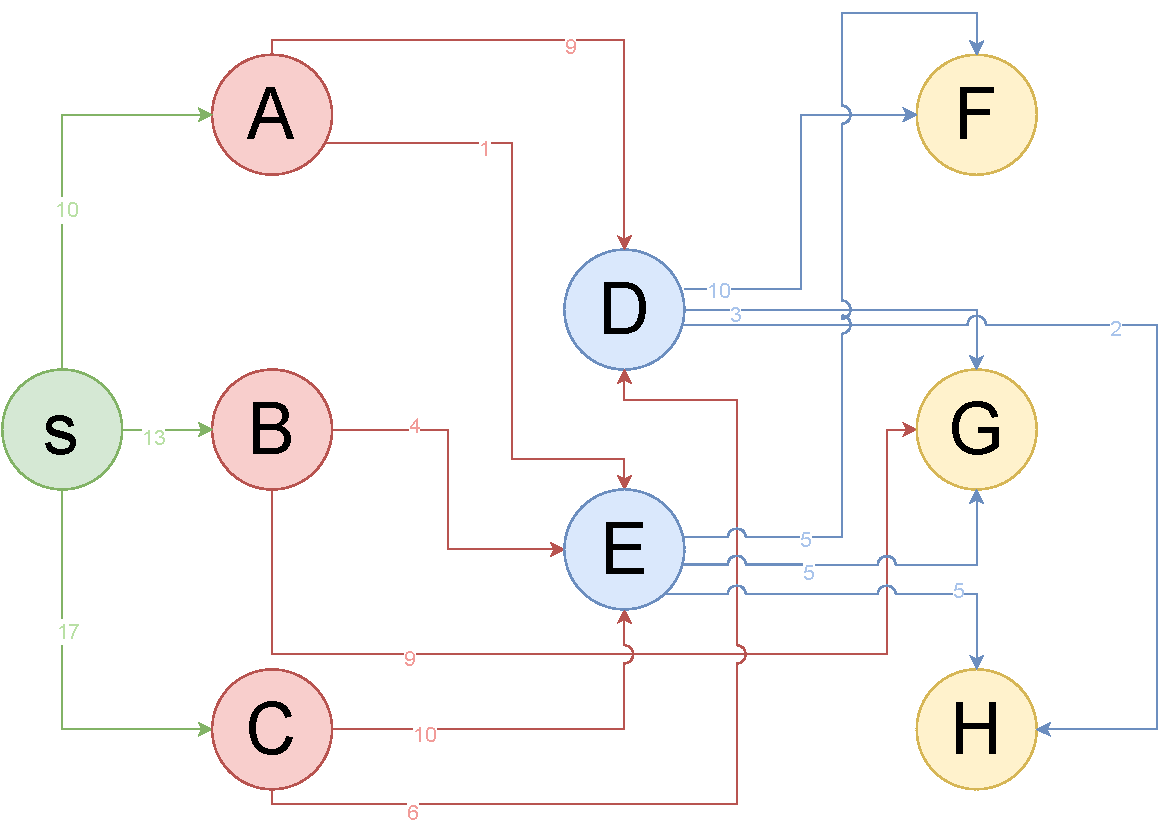
\includepdf[pages=-]{flow12.pdf}

\paragraph{Wnioski}
Następujące przepływy są zbyt niskie w porównaniu do przepustowości:
\[ p_{AD} = 9 \le 15  \]
\[ p_{AE} = 1 \le 10  \]
\[ p_{BE} = 4 \le 9  \]
\[ p_{CD} = 6 \le 20  \]
Zwiększenie przepływów do poziomu maksymalnej przepustowości zwiększyło by wydajność sieci



